\documentclass[sansserif]{beamer}

\mode<presentation>
{
%  \usetheme{Berlin}
%%%  \usecolortheme{lily}
%  \usecolortheme{usyd}
%  \useinnertheme{rectangles}
%  \useoutertheme[subsection=false]{smoothbars}

%  \usenavigationsymbolstemplate{}
%  \setbeamercovered{transparent}
\usepackage{beamerthemesplit}
\usetheme{lankton-purple}
}

\newcommand{\p}{\item}
\newcommand{\bpoints}{\begin{itemize}}
\newcommand{\epoints}{\end{itemize}}

\usepackage{multirow}
\usepackage{ragged2e}
\usepackage[T1]{fontenc}		% Font
%%%\usepackage[scaled]{libertine}	% Biolinum type
\usepackage[scaled]{berasans}	% Bera Sans type

%\title[\hspace{28.5em} \insertframenumber/14]
%\title[Distil \hspace{24.8em} \insertframenumber/13]
\title[Distil \hspace{24.8em}]
{Distil: a \underline{Dist}ributed \underline{I}nformation \underline{L}ibrary
\\\vspace{1em}{\small a document, bibliography, and research knowledge
management system, built on top of Git}}

\author[James Boyden]
{\\{\large \textbf{James Boyden}}}

\date{{\tiny 20th of April, 2011}}
%\date{}

\begin{document}

\begin{frame}
	\titlepage
\end{frame}

\begin{frame}{Why I'm presenting this}
	\begin{itemize}
		\item I find it useful to organise the papers I read.
		\\ \hspace{2em} $\Rightarrow$ It might be useful to you too. \vspace{1em}
		\item It's Open Source software.
		\\ \hspace{2em} $\Rightarrow$ I welcome any additions or bugfixes.
		\\ \hspace{5.5em} (Yes, it's written in Python.)
	\end{itemize}
\end{frame}

\begin{frame}{What Distil is}
	Two main components:
	\begin{itemize}
		\item a command-line tool ({\tt distil}) to import new bibs \& docs
		\item a Trac-inspired note-management wiki
	\end{itemize}

	\begin{center}
		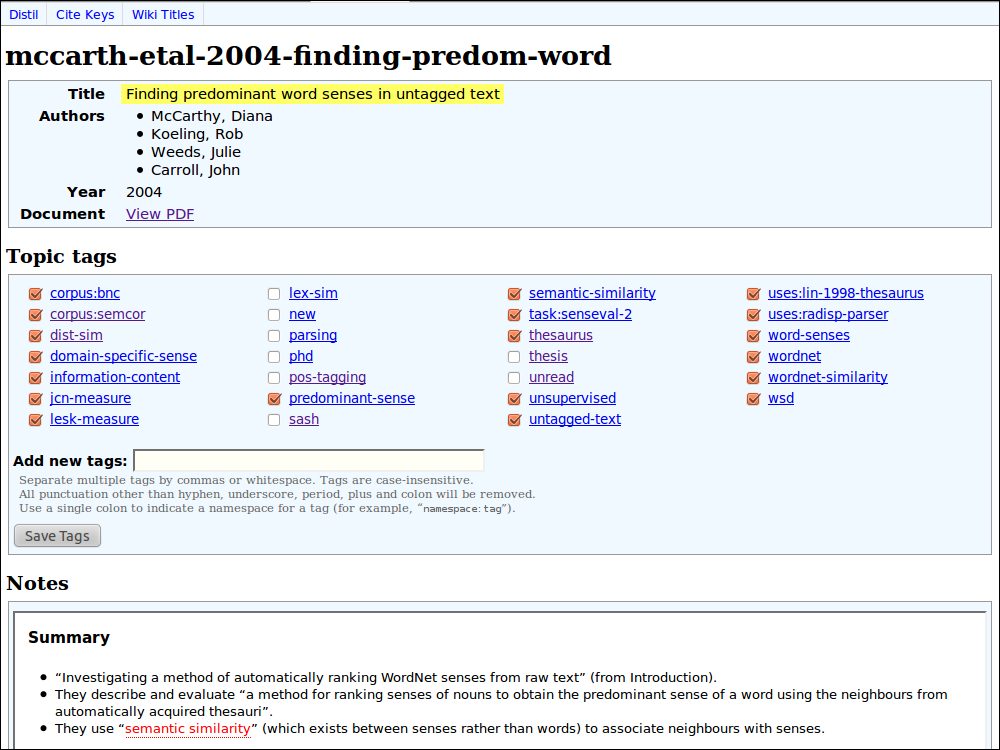
\includegraphics[width=8cm]{screenshot.png}
	\end{center}
\end{frame}

\begin{frame}{Why I built it}
	I wanted a system that...
	\begin{itemize}
		\item could store docs internally (PDF, DOC, PS.GZ, etc.)
		\item could synchronise easily
		\begin{itemize}
			\item between home and uni
			\item or to a backup location
			\item asynchronously
		\end{itemize}
		\item allowed me to take notes easily
		\begin{itemize}
			\item in a wiki-like syntax
			\item with inter-note wiki-links
			\item using Vim keybindings (or Emacs!)
		\end{itemize}
		\item allowed me to tag/label easily
		\item incorporated version control
	\end{itemize}
\end{frame}

\begin{frame}{Why I built it, part 2}
	I wanted a system that...
	\begin{itemize}
		\item could import new bibs \& docs quickly and easily
		\item understood BibTeX
		\item could auto-generate consistent BibTeX cite-keys
		\begin{itemize}
			\item which were also mnemonic
			\item but not \textit{too} long
		\end{itemize}
		\item could work without a network connection
		\item allowed me to view/edit multiple items simultaneously
		\item was Unicode-friendly
	\end{itemize}
\end{frame}

\begin{frame}{Some disclaimers}
	\begin{itemize}
		\item ``Agile'' development methodology
		\\ \hspace{2em} $\Rightarrow$ very feature-incomplete \vspace{1em}
		\item Definitely ``alpha'' software
	\end{itemize}
\end{frame}

\begin{frame}{Some assurances}
	\begin{itemize}
		\item I use it every day \vspace{1em}
		\item Built upon the stable foundation of Git
		\begin{itemize}
			\item If it fails halfway through an operation (rare)
			\\ \hspace{2em} $\Rightarrow$ revert/complete the uncommitted changes \vspace{1em}
			\item If it commits something wrong (never happened yet)
			\\ \hspace{2em} $\Rightarrow$ revert the changeset \vspace{1em}
			\item The Git wrapper functions are simple and well-tested \vspace{1em}
			\item No database lockups/corruption!
		\end{itemize}
	\end{itemize}
\end{frame}

\begin{frame}{The {\tt distil} command}

	{\tt distil somefoo.bib otherbar.pdf whatever.abs} \vspace{2em}
	\begin{itemize}
		\item Command-line arguments:
		\begin{enumerate}
			\item a BibTeX \textbf{bibliography}
			\item the \textbf{document} (pdf, doc, ps.gz, etc.) \textit{(optional)}
			\item a plain-text \textbf{abstract} \textit{(optional)}
		\end{enumerate} \vspace{1em}
		\item What happens:
		\begin{enumerate}
			\item Read the BibTeX file, auto-generate a cite-key
			\item Create a new directory in the repository
			\item Move the files into the new directory
			\item Rename the files
			\item Update the cite-key in the BibTeX file
			\item Git commit
		\end{enumerate}
	\end{itemize}
\end{frame}

\begin{frame}{The cite key}
	\begin{itemize}
		\item Auto-generated from the BibTeX file:
		\begin{itemize}
			\item (at most) \textbf{2 author} components
			\item \textbf{year}
			\item (at most) first \textbf{3 title} components
		\end{itemize}
		\item For example:
		\\ \hspace{1em}{\small ``Finding predominant word senses in untagged text''}
		\\ \hspace{2em}{\small by McCarthy et al (2004)}
		\\ becomes:
		\\ \hspace{2em}{\tt mccarth-etal-2004-finding-predom-word} \vspace{1em}
		\item Actual examples!
		\begin{itemize}
			\item {\tt mccarth-etal-2004-automat-acquir-predom}
			\item {\tt mccarth-etal-2004-automat-identif-infreq}
			\item {\tt mccarth-etal-2004-finding-predom-word}
			\item {\tt mccarth-etal-2004-ranking-wordnet-senses}
		\end{itemize}
	\end{itemize}
\end{frame}

\begin{frame}{The wiki}
	\begin{center}
		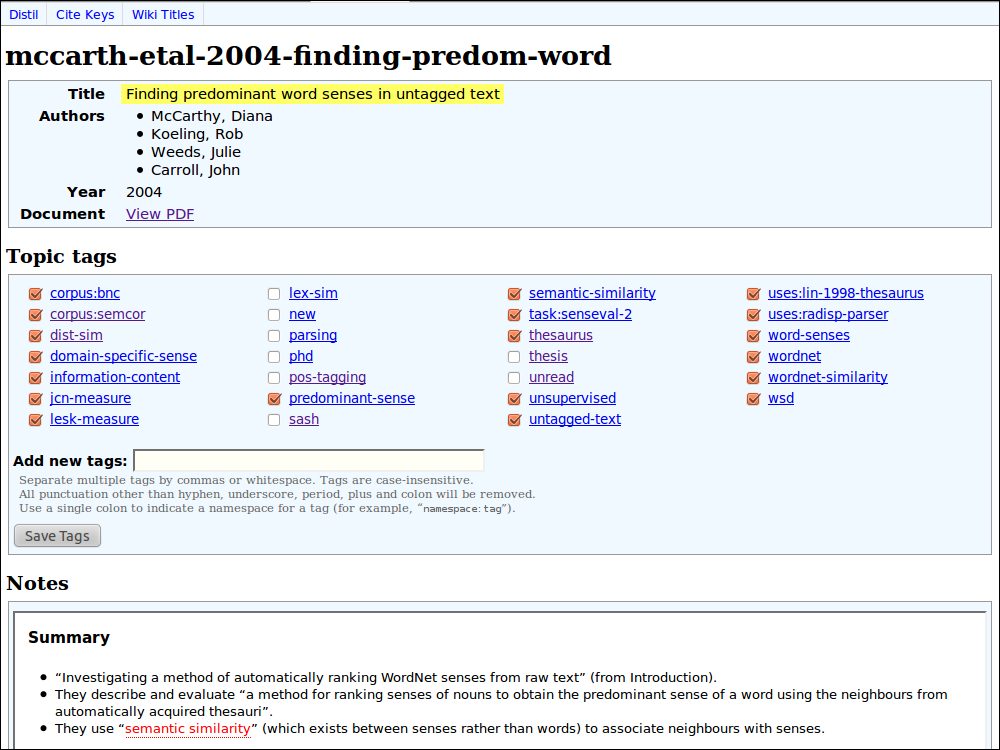
\includegraphics[width=8cm]{screenshot.png}
	\end{center}
	\begin{center}
		\url{http://pc-4e32-1.it.usyd.edu.au:8888/}
	\end{center}
\end{frame}

\begin{frame}{What we have today}
	\begin{itemize}
		\item Importing bibs, docs, abstracts
		\item Auto-generating cite-keys
		\item Git wrapper functions
		\item Wiki for notes on bibs and topics
		\begin{itemize}
			\item wiki-markup
			\item inter-wiki links (including inter-bib ``cite'' links)
		\end{itemize}
		\item Topic-tagging of bibs
		\item Indexes of tags and cite-keys
	\end{itemize}
\end{frame}

\begin{frame}{Some potential future features}
	\begin{itemize}
		\item Topic-tagging wiki pages
		\item Attachments
		\item {\tt /timeline}
		\item Creating/editing BibTeX bibliographies
		\item Better support for LateX in BibTeX
		\item Indexing/search
		\item Track-backs
		\begin{itemize}
			\item Links to this page.
			\item This paper was cited by \textit{X}.
			\item \textit{X} said ``Interesting comment'' about this paper.
		\end{itemize}
		\item {\tt /authors/curran/j*}
		\item \textit{Actually} being distributed
		\\ {\small (between people in a team, not just different computers)}
	\end{itemize}
\end{frame}

\begin{frame}{Thank you}
	\begin{center}
		{\Huge Any questions?}
	\end{center}
\end{frame}

\end{document}
